\section{DATASET}
\label{sec:dataset}

\subsection{Fleet of Cars}
The dataset was collected using a fleet of 1/10th scale RC model cars (\Cref{fig:fleet}) similar to that of \cite{intel_paper, williams2017information, giusti2016machine, muller2006off, muller2013real, krasheninnikov2017autonomous} for recording data in unstructured off-road environments as well as sidewalks. \Cref{fig:cars} shows the main sensor and control components of the car. The small size of the model car provides the flexibility to experiment in diverse driving terrains and lighting conditions. Our dataset contains hundreds of hours of data from environments including city sidewalks, parks, forests and snowy environments. Data were collected in different weather conditions and at different times of the day (\Cref{fig:diverse}). Additionally, the small size of the cars allow for experiments with atypical driving behaviors and the collection of data involving the vehicle making and recovering from mistakes.

There are four computing nodes in the car -- one NVIDIA Jetson TX1 \footnote{ TX1 Developer Kit at \url{https://developer.nvidia.com/embedded/buy/jetson-tx1-devkit}} and three Arduino Uno\footnote{Arduino Unos available at \url{https://www.arduino.cc/}} micro-controllers.

The nodes communicate with one another using Robot Operating System (ROS) Kinetic \cite{quigley2009ros}. Arduino \#1 performs pulse width modulation for the steering servo motor and power control of the DC drive motor. It also connects to an RC receiver, through which user steering and drive power commands from the RC transmitter are received. Arduino \#1 provides the RC controller data to the TX1 and receives servo position and motor power information in return. The main sensor for the car is the ZED RGB stereo camera, developed by StereoLabs\footnote{ ZED Stereo Camera from \url{https://www.stereolabs.com/zed/specs/}}, connected to the TX1. There are optional auxiliary sensors, such as the gyroscope and accelerometer, which are controlled by Arduino \#2, although no auxiliary sensors were used for the experiments described in this paper. Arduino \#3 is dedicated to real-time debug message display using an 8x8 LED panel. 

During the data collection process, the car is controlled using an RC Transmitter. Every 33 ms, the left and right RGB images from the stereo camera, along with steering position and motor power level, are saved to on-board SSD storage. The datasets are labelled according to the behavioral mode and operation mode used.

\subsection{Behavioral Modes}

The dataset also contains annotated modes of behavior for the model car to constitute the behavioral modes used during inference for the MultiNets. We use three distinct behavioral driving modes:

\begin{enumerate}
    \item \textbf{Direct Mode} consists of data with the car driving with few obstructions or obstacles, usually on a winding sidewalk or forest path (\Cref{fig1:direct}).
    \item \textbf{Follow Mode} consists of data with the car following a lead car in front of it. In this mode, speed modulation occurs as maintaining an uniform distance from the lead car is attempted during driving (\Cref{fig1:follow}).
    \item \textbf{Furtive Mode} consists of data where the car attempts to drive slowly in close proximity to perceived boundaries e.g.\ shrubbery or bushes on either side of a path. If no such boundaries are identified, the car speeds up along the path until one is found (\Cref{fig1:furtive}).
\end{enumerate}

%\begin{figure}[t]
%   \centering
%   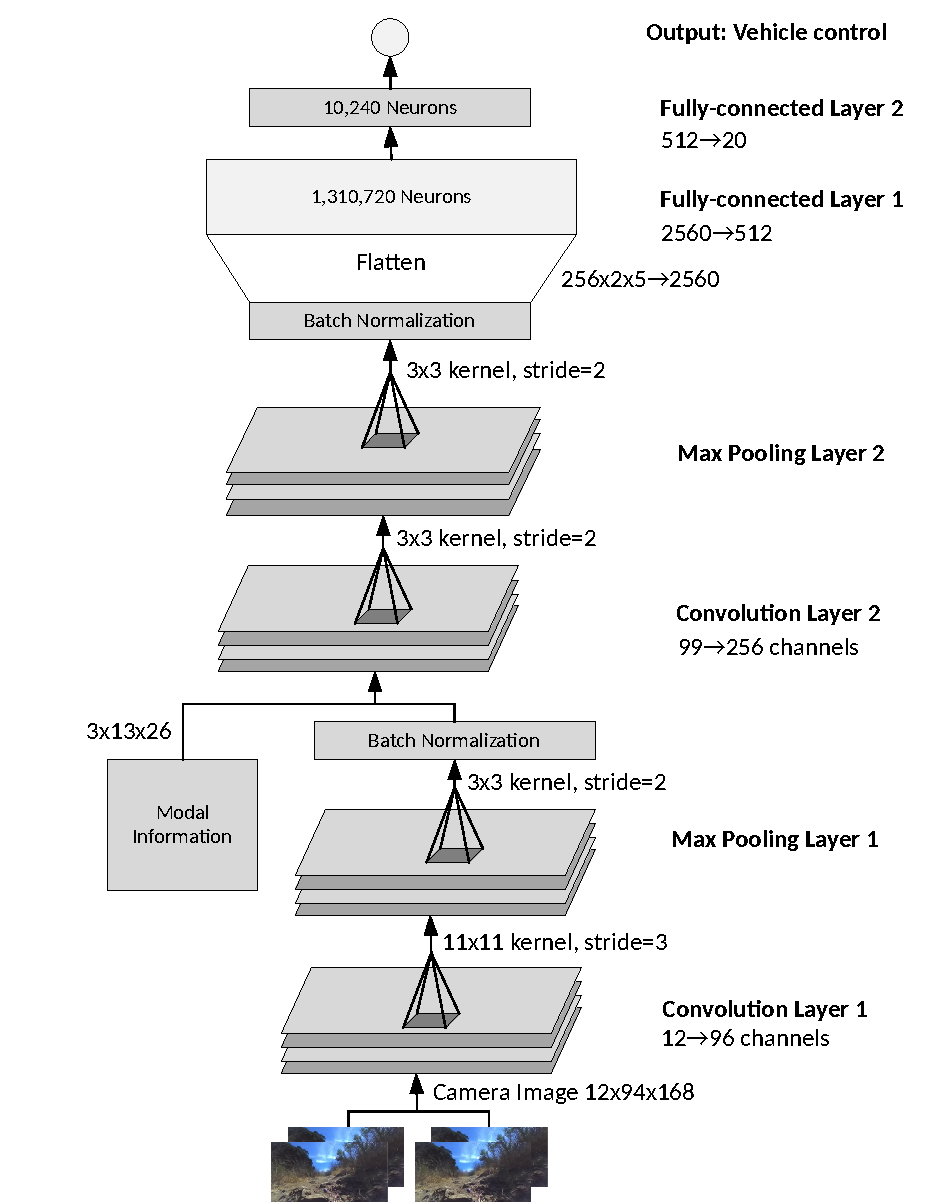
\includegraphics[width=\columnwidth]{paper/content/images/z2color}
%   \caption{Z2Color Network Architecture with Privileged Modal Insertion}
%   \label{fig:squeeze}
%\end{figure}
%

\subsection{Operation Modes}
During data collection runs, the car operates in one of three operational modes: \textit{autonomous}, \textit{expert}, and \textit{correctional}. The autonomous mode is used for evaluating trained networks by allowing a trained network to infer the speed and steering of the model car from the input camera data. During the autonomous mode, the RC receiver remains active, allowing the user to manually override the network's predicted steering values when needed. If a human expert monitoring the car adjusts the speed or steering on the RC transmitter, the car will automatically move into correctional mode allowing for human correction and recovery to avoid the car flipping over or hitting an obstacle. Finally, in the expert mode the expert has full control of the vehicle and records data for future imitation learning.

\subsection{Dataset Aggregation}
Our system utilizes imitation learning. Imitation learning has a basic problem, known as the data mismatch problem, which occurs when a trained network encounters new situations which aren't represented in the dataset of expert driving. In this situation, error compounds quadratically over time to bring the network farther away from expert trajectory \cite{ross2010efficient}.

To solve this problem we implemented a novel approach to the DAgger algorithm \cite{ross2011reduction} which traditionally requires manual labeling of expert trajectories after data are collected from the running network. The small size of the car allowed us to safely record data of the RC vehicle making and recovering from mistakes. New data are then merged with the active dataset for future training in the next iteration. Due to the live corrections, we are able to streamline the data collection process by solving the data mismatch problem while eliminating the need for expert labeling after the data are collected. Our dataset consisted of 19.24\% correctional data and 80.76\% expert data at the time of training and evaluation of the models presented in this paper.

\subsection{Data Moments}

The ROS system gathers time stamps for recorded motor, steer, and camera data. After this data are collected it is processed, interpolated, and synchronized into packets we call \textit{data moments}. We define a data moment as a set of four RGB input images and an associated collection of ten drive speed and steering angle values. Our networks are trained and evaluated on   series of data moments. A data moment associates the input camera images to motor power and steering angles which when actuated create a spatial trajectory for the car to follow (\Cref{fig:moment}). 

\begin{figure}
\centering
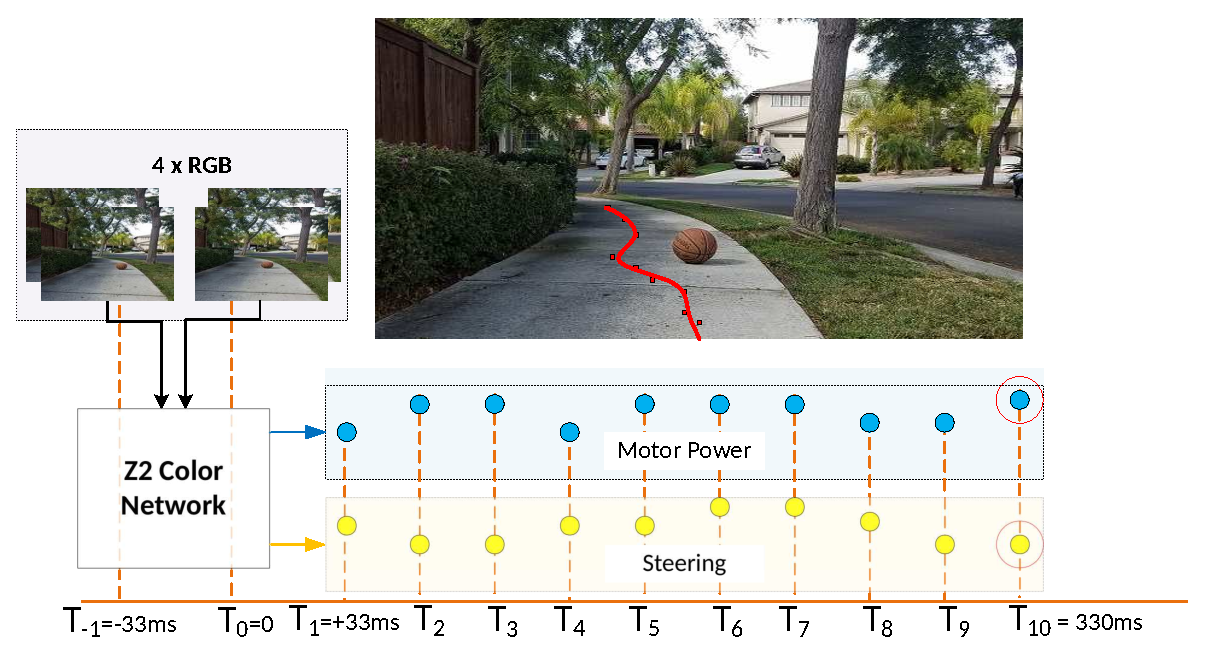
\includegraphics[width=\columnwidth]{paper/content/images/data_moment}
\caption{Data Moment}
\label{fig:moment}
\end{figure}

For perception of depth, we use left and right images from the stereo camera. To allow the network to perceive motion we use image pairs from two time steps -- one image pair gives the current position of the car, and the other is from 33 ms in the past. This way each data moment contains four RGB images.

Motor, steering, and image data are collected and stored from the car every 33 ms.
The latency between the network's prediction and actuation on the vehicle is 330 ms to mimic human reaction time. Thus the network predicts 330 ms into the future to account for this delay.

Rather than only training the network to predict a single steering and drive speed value 330 ms into the future, we instead utilize multi-task learning to improve the network's performance. To accomplish this, we train the networks to predict 10 future time steps, each 33 ms apart. In this case, only the 10th value is used for actuation and inference, while the other values serve as side-tasks to improve the cars understanding of the scene and performance on the actuated values.

The steering and motor values are floating point values ranging from zero to one. In the case of the motor values, one represents a full speed of approximately 9 meters per second. A value of zero for the motors is full speed in reverse; backward driving is used occasionally for abrupt stopping. For steering, a value of one represents the maximum steering angle towards the right, while a value of zero is the maximum steering angle towards the left.

While it is well known that the addition of such side-tasks benefits learning \cite{caruana1998multitask}, we qualitatively confirmed these improvements through on-the-road experiments. In these experiments, networks predicting only final actuation values were compared with MTL networks. It was observed that the MTL networks required far less manual correction and had greater autonomy, suggesting that the side tasks provide the network improved spatial awareness and driving capability.
